\documentclass{article}
\usepackage[utf8]{inputenc}
\usepackage{tikz}
\usepackage{amsmath}
\usepackage{graphicx}
\usepackage[margin=0.05in,paperwidth=12in,paperheight=6in]{geometry}

\usetikzlibrary{shapes.geometric, arrows}


\begin{document}
\LARGE
\begin{minipage}{.475\linewidth}
	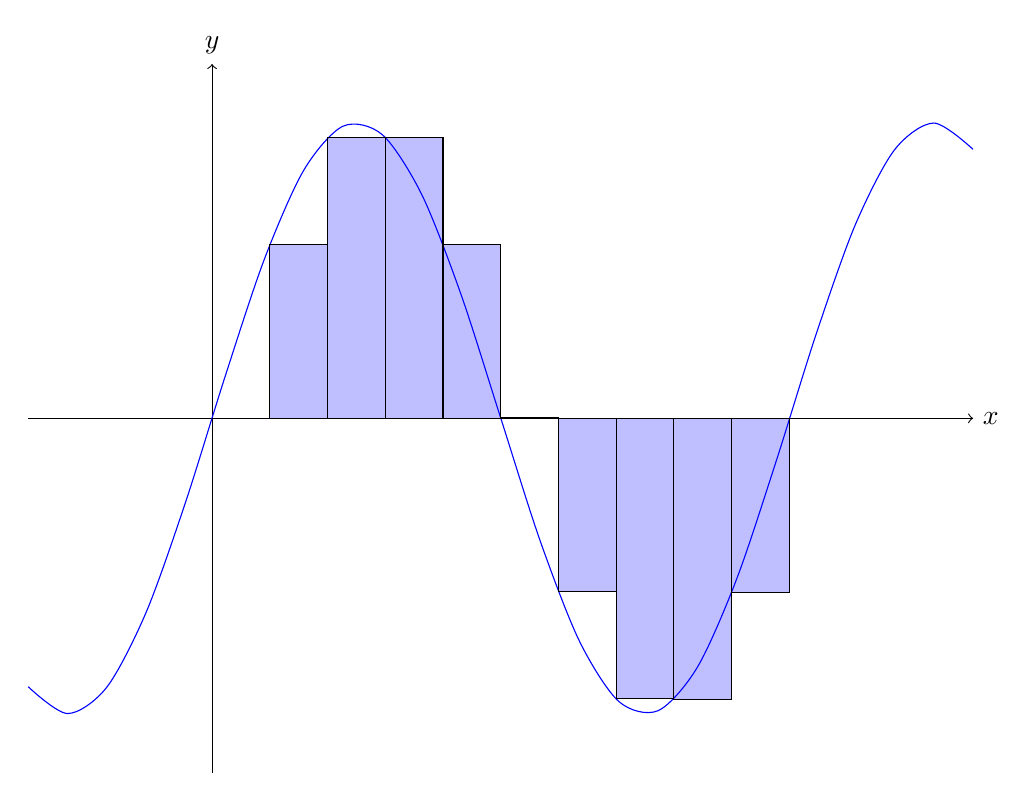
\begin{tikzpicture}[xscale=2.3346303501945522,yscale=7.50001189007053]
	  \draw[->] (-1,0) -- (4.140000000000001,0) node[right] {$x$};
	  \draw[->] (0,-0.599998414659837) -- (0,0.599999682931895) node[above] {$y$};
  
	  \draw[domain=-1:4.140000000000001,smooth,variable=\x,blue] plot ({\x},{sin((\x) r)*cos((\x) r)});
	  \draw[fill=blue, draw=black, fill opacity=0.25] (0.0,0) rectangle (0.314,0);
\draw[fill=blue, draw=black, fill opacity=0.25] (0.314,0) rectangle (0.628,0.293763762856946);
\draw[fill=blue, draw=black, fill opacity=0.25] (0.628,0) rectangle (0.942,0.475429730253235);
\draw[fill=blue, draw=black, fill opacity=0.25] (0.942,0) rectangle (1.256,0.475675688116914);
\draw[fill=blue, draw=black, fill opacity=0.25] (1.256,0) rectangle (1.57,0.294407780983898);
\draw[fill=blue, draw=black, fill opacity=0.25] (1.57,0) rectangle (1.884,0.000796326458243414);
\draw[fill=blue, draw=black, fill opacity=0.25] (1.884,0) rectangle (2.198,-0.293118999585014);
\draw[fill=blue, draw=black, fill opacity=0.25] (2.198,0) rectangle (2.512,-0.475182566440688);
\draw[fill=blue, draw=black, fill opacity=0.25] (2.512,0) rectangle (2.826,-0.475920439407843);
\draw[fill=blue, draw=black, fill opacity=0.25] (2.826,0) rectangle (3.14,-0.295051052332288);

	\end{tikzpicture}
	\end{minipage}\hfill
\begin{minipage}{.5\linewidth}
	\scalebox{1.45}{\parbox{.5\linewidth}{%
	\large
	\begin{align*}
\displaystyle\int_{0}^{3.14} f(x) dx & \approx A(r_1)+A(r_2)+\dots+A(r_{10})\\
& \approx w\cdot h(r_1)+w\cdot h(r_2)+\dots+w\cdot h(r_{10})\\
& \approx w\cdot (h(r_1)+h(r_2)+\dots+h(r_{10}))\\
& \approx 0.314(f(x_1)+f(x_2)+\dots+f(x_{10}))\\
& \approx 0.314(0+0.29+\dots-0.3)\\
& \approx 0\\
	\end{align*}
	}}
	\end{minipage}
\begin{minipage}{.475\linewidth}
	\huge
	\vspace{5pt}
	\noindent
	Approximate the area under the curve $f(x)=\sin{\left (x \right )} \cos{\left (x \right )}$ on the interval $[0,3.14]$ with $10$ rectangles of equal width using the LRAM method.
	\begin{center}
	\begin{tabular}{ |c|c|c|c| } 
		\hline
		$a=0$ & $b=3.14$ & $n=10$ & $w=\frac{b-a}{n}=0.314$\\ 
		\hline
		\end{tabular}
	\end{center}
	\end{minipage}\hfill
\begin{minipage}{.5\linewidth}
	\huge
	\vspace{5pt}
	\begin{center}
	\Large
	\begin{tabular}{ |c|c|c|c|c|c|c|c|c|c|c| } 
	 \hline
	 i & 1 & 2 & 3 & 4 & 5 & 6 & 7 & 8 & 9 & 10\\ 
	 \hline
	$x_i$ & 0 & 0.31 & 0.63 & 0.94 & 1.26 & 1.57 & 1.88 & 2.2 & 2.51 & 2.83\\ 
	\hline
	$f(x_i)$ & 0 & 0.29 & 0.48 & 0.48 & 0.29 & 0 & -0.29 & -0.48 & -0.48 & -0.3\\ 
	\hline
	$A(r_i)$ & 0 & 0.09 & 0.15 & 0.15 & 0.09 & 0 & -0.09 & -0.15 & -0.15 & -0.09\\ 
	 \hline
	\end{tabular}
	\end{center}
	\end{minipage}
	\end{document}